\section{Dynamic Mode Decomposition (DMD)}
Let us go back to the case of a linear dynamical system
\begin{equation*}
    \vb{x}_{n+1} = \vb*{A}\vb{x}_n, \qquad \vb*{A}\in\R^{n\times n}.
\end{equation*}
As already discussed, in order to extract the dynamic characteristics we need to analyze the spectral properties of $\vb{A}$. However, in a data-drive perspective, we cannot assume that we have access to $\vb*{A}$, but only to a sequence of snapshots. Therefore, we are interested in computing the eigenpairs of $\vb{A}$, or at least the dominant ones, from a sequence of snapshots
\begin{equation*}
    \label{krylov_space}
    \vb*{V}_1^N = \left[\vb{v}_1, \vb{v}_2, \dots, \vb{v}_N\right] = \left[\vb{v}_1, \vb*{A}\vb{v}_1, \dots, \vb*{A}^N\vb{v}_1\right].
\end{equation*}
Since the columns of $\vb*{V}_1^N$ span a Krylov subspace, it is natural to apply a Krylov subspace method. As we do not have access to the matrix $\vb*{A}$ and we cannot compute products of vectors by this matrix, we cannot directly apply numerically stable algorithms such as the Arnoldi method, and we can rely only on the sequence of snapshots we are given in input. \emph{Dynamic Mode Decomposition} (DMD) \cite{schmid_dynamic_2010} is a variant of the Arnoldi method that does not require computing multiplications by $\vb*{A}$, nor any knowledge of the matrix. 

Let us first suppose that, after a certain number of iterates, we found an $\vb*{A}$-invariant Krylov subspace and that $\vb{v}_N$ can be expressed as a linear combination of the previous linearly independent snapshots, i.e.
\begin{equation}
    \label{vn_exact}
    \vb{v}_N = a_1 \vb{v}_1 + \dots + a_{N-1} \vb{v}_{N-1} = \vb{V}_1^{N-1}\vb{a}, \qquad \vb{a}\in\R^{N-1}.
\end{equation}
We can rewrite the relation in \eqref{vn_exact} as:
\begin{equation*}
    \vb*{A}\vb*{V}_1^{N-1} = \vb*{V}_2^{N} = \vb*{V}_1^{N-1}\vb*{S}
\end{equation*}
where $\vb*{S}$ is the companion matrix associated with $\vb{a}$, defined by:
\begin{equation}
    \label{S_definition}
    \vb*{S} :=
   \begin{bmatrix}
   0     &        &       &      & a_1 \\
   1     & 0      &       &      & a_2 \\
         & \ddots & \ddots&      & \vdots \\ 
         &        & 1     & 0    & a_{N-2} \\
         &        &       & 1    & a_{N-1} \\
   \end{bmatrix}.
\end{equation}
The eigenvalues of $\vb*{S}$ are also eigenvalues of $\vb*{A}$. Indeed, if $\vb*{S}\vb{x} = \lambda \vb{x}, \,\, \vb{x}\neq 0$ then $\vb{y} = \vb{V}_1^{N-1}\vb{x}\neq 0$ (we assumed that the first $N-1$ snapshots are linearly independent) and $\vb*{A}\vb{y} = \vb*{A}\vb{V}_1^{N-1}\vb{x} = \vb{V}_1^{N-1}\vb*{S}\vb{x} = \lambda \vb{V}_1^{N-1}\vb{x} = \lambda \vb{y}$.

In general, $\vb{v}_N$ does not necessarily belong to the Span of the columns of $\vb*{V}_1^N$. However, as $N$ increases the snapshots tend to lie in the same direction (or at least in the same subspace) and we can expect that after a critical number of snapshots $\vb{v}_N$ \emph{almost} lies in the $\Span{(\vb*{V}_1^{N-1})}$, where by \emph{almost} we mean that the normalized difference between $\vb{v}_N$ and its projection onto $\Span{(\vb*{V}_1^{N-1})}$ is small. Therefore, again assuming that the previous vectors are linearly independent, we we want to write
\begin{equation}
    \label{vn_error}
    \begin{split}
        & \vb{v}_N = a_1 \vb{v}_1 + \dots + a_{N-1} \vb{v}_{N-1} + \vb{r}, \qquad \text{i.e.}\\
        & \vb*{A}\vb*{V}_1^{N-1}  = \vb*{V}_1^{N-1}\vb*{S} + \vb{r}\vb{e}_{N-1}^T
    \end{split}
\end{equation}
so that we minimize the norm of the residual $\vb{r} = \vb{v}_N - \vb*{V}_1^{N-1}\vb{a}$. To solve the corresponding least square problem, we compute the thin QR-decomposition of $\vb*{V}_1^{N-1} = \vb*{Q}\vb*{R}$ and then we obtain
\begin{equation}
    \label{a_qrleastsquare}
    \vb{a} = \vb*{R}^{-1} \vb*{Q}^*\vb{v}_N.
\end{equation}
The eigenvalues $\{\lambda_j\}_{j = 1}^{N-1}$ of the companion matrix $\vb*{S}$ are now approximations of the eigenvalues of $\vb*{A}$ and are called \emph{Ritz values}. The corresponding approximated eigenvectors $\vb{y}_j = \vb*{V}_1^{N-1}\vb{x}_j$, where $\vb{x}_j$ is an eigenvector of $\vb*{S}$ are the so called \emph{Ritz vectors}.

The above mentioned method was the original version of the DMD \cite{schmid_dynamic_2010}. However, even if it mathematically correct and equivalent to the Arnoldi method in exact arithmetic (see \Cref{section_dmd_arnoldi}), an implementation using the companion matrix $\vb*{S}$ gives rise to a numerically unstable algorithm that is usually not capable to extract more than one or two dominant eigenpairs. Using the Singular Value Decomposition (SVD) it is possible to obtain a mathematically equivalent but better-conditioned algorithm, which might be particularly useful when $\vb*{V}_1^{N-1}$ is close to singular (it is very likely to happen for large $N$). This second version of the DMD is what nowadays is referred as DMD. Suppose that we computed a SVD of the snapshots matrix
\begin{equation*}
    \vb*{V}_1^{N-1} = \vb*{U}\vb*{\Sigma}\vb*{W}^* \qquad \vb*{\Sigma}\in\R^{N-1\times N-1},
\end{equation*}
we can now rewrite \eqref{vn_error} as
\begin{equation}
    \label{vn_error_rewritten}
    \vb*{A}\vb*{U}\vb*{\Sigma}\vb*{W}^* = \vb*{U}\vb*{\Sigma}\vb*{W}^*\vb*{S} + \vb{r}\vb{e}_{N-1}^T = \vb*{V}_2^N
\end{equation}
and rearranging
\begin{equation}
    \label{S_tilde_definition}
    \vb*{U}^*\vb*{A}\vb*{U} = \vb*{U}^*\vb*{V}_2^N\vb*{W}\vb*{\Sigma}^{-1} =: \widetilde{\vb*{S}}.
\end{equation}
Once we have computed the eigenpairs $\{(\lambda_j, \vb{x}_j)\}_j$ of the matrix $\widetilde{\vb*{S}}$, which in this case is a full matrix and not of companion type, we obtain the Ritz values and vectors as $\{(\lambda_j, \vb*{U}\vb{x}_j)\}_j$. 

Besides the better conditioning, a great advantage of the SVD-based approach over the Arnoldi-based one is the opportunity to account for rank deficiency in $\vb*{V}_1^{N-1}$ and noise in the data by truncating the SVD of $\vb*{V}_1^{N-1}$. As observed in \cite{schmid_dynamic_2010}, without the use of TSVD it can be difficult to extract more than the first one or two dominant dynamic modes when using data from experiments, as the problem is ill-conditioned. 

As previously mentioned, the two approaches are equivalent since $\vb*{S}$ and $\widetilde{\vb*{S}}$ are linked through a similarity transformation. The residual of the least squares solution is orthogonal to the columns of $\vb*{U}$, hence from \eqref{vn_error_rewritten} and \eqref{S_tilde_definition}:
\begin{equation*}
    \begin{split}
    \widetilde{\vb*{S}} & =
    \vb*{U}^*\vb*{V}_2^N\vb*{W}\vb*{\Sigma}^{-1} =
    \vb*{U}^*(\vb*{U}\vb*{\Sigma}\vb*{W}^*\vb*{S} + \vb{r}\vb{e}_{N-1}^T)\vb*{W}\vb*{\Sigma}^{-1} = \\
    & = (\vb*{\Sigma}\vb*{W}^*) \vb*{S} (\vb*{W}\vb*{\Sigma}^{-1}) =
    (\vb*{\Sigma}\vb*{W}^*) \vb*{S} (\vb*{\Sigma}\vb*{W}^*)^{-1}    
    \end{split}
\end{equation*}

The SVD-based version of DMD is summarized in \Cref{alg_dmd}.

\begin{algorithm}
\caption{\textbf{SVD-based DMD}}
\label{alg_dmd}
\textbf{Input:} $\vb{v}_1,\dots, \vb{v}_N$
\begin{algorithmic}[1]
\State Define the matrices $\vb*{V}_1^{N-1} = \left[\vb{v}_1,\dots,\vb{v}_{N-1}\right]$ and $\vb*{V}_2^{N} = \left[\vb{v}_2,\dots,\vb{v}_{N}\right]$.
\State Compute the (eventually truncated) SVD of $\vb*{V}_1^{N-1} = \vb*{U}\vb*{\Sigma}\vb*{W}^*,\,\, \vb*{\Sigma}\in\R^{p\times p}$.
\State Define the matrix $\widetilde{\vb*{S}} := \vb*{U}^*\vb*{V}_2^N\vb*{W}\vb*{\Sigma}^{-1}$.
\State Compute the eigenpairs $\{(\lambda_j, \vb{x}_j)\}_j$ of $\widetilde{\vb*{S}}$.
\State Compute the Ritz vector corresponding to the Ritz value $\lambda_j$ as $\vb{y}_j = \vb*{U}\vb{x}_j$. 
\end{algorithmic}
\textbf{Output:} Ritz values $\lambda_1,\dots,\lambda_{p}$ and corresponding Ritz vectors $\vb{y}_1,\dots, \vb{y}_p$
\end{algorithm}

The DMD algorithm presented above assumes that $\vb{x}_{n+1} = \vb*{A}\vb{x}_n$, i.e. that the system is and it is not clear what the algorithm produces for nonlinear dynamical systems. It can be shown that for nonlinear dynamics, the algorithm outputs, in some sense, approximations of the Koopman modes and associated eigenvalues with respect to a chosen observable \cite{rowley_spectral_2009, tu_dynamic_2014}. However, as discussed in \cite{tu_dynamic_2014}, this method has limitations in the case of nonlinear dynamics and it is, therefore, a better choice to use methods such as Extended DMD \cite{williams_data-driven_2015} (see \Cref{section_edmd}).


\subsection{DMD and the Arnoldi method}
\label{section_dmd_arnoldi}
The Arnoldi method and the DMD are equivalent in exact arithmetic. In the following section, we will discuss and prove this statement, emphasizing why the Arnoldi algorithm is generally more stable.

The Arnoldi method computes an orthonormal basis of the Krylov subspace spanned by the columns of $\vb*{V}_1^{N-1}$ computing the snapshots implicitly. In particular, the algorithm computes a matrix $\vb*{Q}_{N-1} = \left[\vb{q}_1,\dots, \vb{q}_{N-1}\right]$ with columns that form an orthonormal basis of $\Span{(\vb*{V}_1^{N-1})}$ and: 
\begin{enumerate}[label=(\roman*)]
    \item $\vb*{V}_1^{N-1} = \vb*{Q}_{N-1} \vb*{R}_{N-1}$ is a thin QR-decomposition (with $\vb*{R}_{N-1}$ that is computed implicitly);
    \item $\vb*{H}_{N-1} = \vb*{Q}_{N-1}^* \vb*{A} \vb*{Q}_{N-1}$ is a Hessenberg matrix.
\end{enumerate}
Then the eigenpairs approximations are obtained from the eigenpairs of $\vb*{H}_{N-1}$.

This is mathematically equivalent to the DMD algorithm. Indeed from \eqref{vn_error} and \eqref{a_qrleastsquare} the residual $\vb{r}$ can be written as
\begin{equation*}
    \vb{r} = \vb{v}_N - \vb*{V}_1^{N-1}\vb*{R}_{N-1}^{-1}\vb*{Q}_{N-1}^*\vb{v}_N = v_N - \vb*{Q}_{N-1}\vb*{Q}_{N-1}^*\vb{v}_N
\end{equation*}
and therefore $\vb*{Q}_{N-1}^*vb{r} = 0$. Finally plugging the QR-decomposition into \eqref{vn_error}
\begin{equation*}
    \vb*{A}\vb*{Q}_{N-1}\vb*{R}_{N-1} = \vb*{Q}_{N-1}\vb*{R}_{N-1}\vb*{S} + \vb{r}\vb{e}_{N-1}^T
\end{equation*}
and multiplying by $\vb*{Q}_{N-1}^*$ on the left and by $\vb*{R}_{N-1}^{-1}$ on the right
\begin{equation}
    \label{similarity_arnoldi_dmd}
    \vb*{H}_{N-1} = \vb*{Q}_{N-1}\vb*{A}\vb*{Q}_{N-1} = \vb*{R}_{N-1}\vb*{S}\vb*{R}_{N-1}^{-1}.
\end{equation}
Hence $\vb*{H}_{N-1}$ and $\vb*{S}$ are linked through a similarity transformation.

Although the two algorithms are equivalent mathematically and in exact arithmetic, the Arnoldi algorithm is numerically more stable. Indeed, as the number of snapshots increases, the vectors tend to become linearly dependent and therefore, the matrix $V_1^N$ becomes close to singular, hence ill-conditioned. Computing its QR-decomposition and $\vb{a} = \vb*{R}_{N-1}^{-1} \vb*{Q}_{N-1}^*\vb{v}_N$ might produce inaccurate results in floating-point arithmetic. Even if the previously mentioned problem can be partially solved using the SVD-based DMD and performing a truncated SVD, another major problem is intrinsic to the data-driven approach. One of the major strengths of the Arnoldi algorithm is that it does not even compute the vectors $\vb{x}_j = \vb*{A}^j \vb{x}_0$ because errors are already made in these computations. However, in a data-driven perspective, this is not possible since what we are given is a sequence of snapshots and not the matrix $\vb*{A}$. Hence, we trade-off better stability and convergence properties for an algorithm that only relies on $V_1^N$ and is therefore applicable to snapshots experimentally collected.

\section{Extended Dynamic Mode Decomposition (EDMD)}
\label{section_edmd}
The \emph{Extended Dynamic Mode Decomposition} (EDMD), originally presented in \cite{williams_data-driven_2015}, is a method that seeks at approximating the Koopman Operator as a finite dimensional operator and then approximate the Koopman (eigenvalue, eigenfunction, mode) tuples from this finite dimensional approximation. The algorithm requires in input:
\begin{itemize}
    \item a dataset of snapshot pairs of the system state, $\{(\vb{x}_0^{(m)}, \vb{x}_1^{(m)})\}_{m = 1}^M$ with $\vb{x}_1^{(m)} = \vb{F}(\vb{x}_0^{(m)})$;
    \item a dictionary of observables $\mathcal{D} = \{\psi_1, \dots, \psi_K\} \subseteq \mathcal{D}(\mathcal{K})$. Let us define the vector-valued observable $\Psi:\Omega\to\C^{1\times k}$ as $\Psi(x) = [\psi_1(x), \dots, \psi_k(x)]$. The choice of the dictionary $\mathcal{D}$ is not easy and depends on the problem at hand. For the moment, let us assume that $\mathcal{D}$ is rich enough to approximate at least a few of the dominant Koopman eigenfunctions.
\end{itemize}

\subsection{Approximation of $\mathcal{K}$ and its eigenpairs}
Let $\phi\in\Span(\mathcal{D})$, then we can write:
\begin{equation*}
    \phi = \sum_{k=1}^K a_k\psi_k = \Psi\vb{a}, \qquad \vb{a}\in\C^K.
\end{equation*}
We aim at generating $\vb*{K}\in\C^{k\times k}$ finite dimensional approximation of $\mathcal{K}$ such that
\begin{equation}
    \label{k_finite_dimensional}
    \mathcal{K}\vb{\phi} = (\Psi \circ \vb{F})\vb{a} = \Psi\vb*K\vb{a} + r
\end{equation}
where the residual term $r = r(\vb{a}, \vb{x})$ is due to the fact that in general $\Span(\mathcal{D})$ is not $\mathcal{K}$-invariant. To obtain the "best" $\vb*{K}\in\C^{k\times k}$ it is natural to minimize the norm of the point-wise maximum of the residual of all possible $\phi\in\Span(\mathcal{D})$, i.e to solve the following problem \cite{colbrook_rigorous_2021}:
\begin{equation}
    \label{edmd_integral_problem}
    \argmin_{\vb*{K}\in\C^{K\times K}}\int_{\Omega} \max_{\vb{a}\in\C^k \\ \norm{\vb{a}} = 1}\abs{r(\vb{a}, \vb{x})}^2 d\omega(\vb{x}) = 
    \argmin_{\vb*{K}\in\C^{K\times K}}\int_{\Omega} \norm{\Psi(\vb{F}(\vb{x})) - \Psi(\vb{x})\vb*{K}}^2 d\omega(\vb{x}).
\end{equation}

We cannot directly compute the integral, thus we need to use a quadrature rule. We take as quadrature nodes our snapshot data $\{\vb{x}_0^{(m)}\}_{m = 1}^M$ with weights $\{w_m\}_{m = 1}^M$. The discretized problem reads:
\begin{equation}
\label{edmd_discretized_problem}
\begin{split}
    &\argmin_{\vb*{K}\in\C^{k\times k}} \sum_{j=1}^M w_j \norm{\Psi(\vb{F}(\vb{x}_0^{(j)})) - \Psi(\vb{x}_0^{(j)})\vb*{K}}^2 d\omega(\vb{x}) = \\
    = &\argmin_{\vb*{K}\in\C^{k\times k}} \sum_{j=1}^M w_j \norm{\Psi(\vb{x}_1^{(j)}) - \Psi(\vb{x}_0^{(j)})\vb*{K}}^2 d\omega(\vb{x}).
\end{split}    
\end{equation}
If we define the matrices
\begin{align}
\label{w_def}
\vb*{W} = \diag(w_1,\dots,w_M)\in\R_+^{M\times M} \\
\label{psi0_def}
\Psi_0 = \left[\Psi(\vb{x}_0^{(1)})^T,\dots,\Psi(\vb{x}_0^{(M)})^T\right]^T\in\C^{M\times K} \\
\label{psi1_def}
\Psi_0 = \left[\Psi(\vb{x}_1^{(1)})^T,\dots,\Psi(\vb{x}_1^{(M)})^T\right]^T\in\C^{M\times K}
\end{align}
we can write the weighted least-square problem in \eqref{edmd_discretized_problem} as 
\begin{equation}
    \label{edmd_discretized_problem_matrix}
    \argmin_{\vb*{K}\in\C^{k\times k}}\norm{\sqrt{\vb*{W}}(\Psi_1 - \Psi_0\vb*{K})}_F^2.
\end{equation}
Since this is a convex problem in $\vb*{K}$, it suffices to impose that the derivative (of the real and of the imaginary part) is zero, from which we get
\begin{equation}
    \label{discretized_problem_solution}
    (\Psi_0^*\vb*{W}\Psi_0)\vb*{K} = \Psi_0^*\vb*{W}\Psi_1 \,\,\Longrightarrow\,\, \vb*{K} = (\Psi_0^*\vb*{W}\Psi_0)^{\dagger}(\Psi_0^*\vb*{W}\Psi_1).
\end{equation}

To approximate the eigenvalue-eigenfunction pair of the Koopman Operator, we use the eigenpairs of its finite dimensional approximation $\vb*{K}$. If $\lambda_j$ is an eigenvalue of $\vb*{K}$ with eigenvector $\bm{\xi}_j$, an approximation of an eigenvalue-eigenfunction pair of $\mathcal{K}$ is $(\lambda_j, \phi_j = \Psi\bm{\xi}_j)$.

A few final remarks for practical implementation of EDMD:
\begin{itemize}
    \item by reducing the size of the dictionary, we may assume without loss of generality that the matrix $(\Psi_0^*\vb*{W}\Psi_0)$ is non-singular. However, we might also consider using TSVD when computing its pseudo-inverse in practice.  
    \item Instead of computing the matrix $\vb*{K} = (\Psi_0^*\vb*{W}\Psi_0)^{\dagger}(\Psi_0^*\vb*{W}\Psi_1)$ and then its eigenpairs, it is often numerically more stable to solve the generalized eigenvalue problem $(\Psi_0^*\vb*{W}\Psi_0)\bm{\xi} = \lambda(\Psi_0^*\vb*{W}\Psi_1)\bm{\xi}$.
\end{itemize}

\subsection{Approximation of the Koopman modes for the full state observable}
Let us consider the full state observable
\begin{equation}
    \label{full_state_def}
    \vb{g}(\vb{x}) = 
    \begin{bmatrix}
    g_1(\vb{x}) \\
    \vdots \\
    g_d(\vb{x})
    \end{bmatrix} = 
    \begin{bmatrix}
    \vb{e}_1^*\vb{x} \\
    \vdots \\
    \vb{e}_d^*\vb{x}
    \end{bmatrix} = \vb{x}.
\end{equation}
Let us assume that $g_i\in\Span(\mathcal{D})$ for all $i = 1,\dots,d$. If this is not the case an intermediate step to project $g_i$ onto $\Span(\mathcal{D})$ is required, with the accuracy strongly depending on the choice of the dictionary. If $g_i\in\Span(\mathcal{D})$ we can write
\begin{equation}
    g_i = \sum_{k=1}^K b_{ki}\psi_k = \Psi\vb{b}_i
\end{equation}
and in matrix form
\begin{equation*}
    \vb{g} = \vb*{B}^T\Psi^T = (\Psi\vb*{B})^T, \qquad \vb*{B} = \left[\vb{b}_1, \dots,\vb{b}_d\right]\in\C^{k\times d}.
\end{equation*}

Let $\bm{\Xi} = \left[\bm{\xi}_1,\dots,\bm{\xi}_K\right]$ be the matrix of the eigenvectors of $\vb*{K}$, the vector of approximate Koopman eigenfunctions $\Phi(\vb{x}) = \left[\phi_1(\vb{x}), \dots, \phi_K(\vb{x})\right]$ can be written as $\Phi = \Psi\bm{\Xi}$. Thus
\begin{equation}
    \vb{g} = \vb*{B}^T\Psi^T = \vb*{B}^T(\bm{\Xi}^T)^{-1}\Phi^T = (\bm{\Xi}^{-1}\vb*{B})^T\Phi^T.
\end{equation}
Since $\bm{\Xi}$ is the matrix of the eigenvectors of $\vb*{K}$, its inverse is $\bm{\Xi}^{-1} = \left[\vb{u}_1, \dots, \vb{u}_K\right]$ where $\vb{u}_i$ is the left eigenvector of $\vb*{K}$ also associated with $\lambda_i$ and appropriately scaled so that $\vb{u}_i^*\bm{\xi}_i = 1$. We can therefore compute the left eigenvectors of and letting  $\vb*{V} = (\vb*{U}^*\vb*{B})^T$, then
\begin{equation}
    \vb{g} = \vb*{V}\Psi^T = \sum_{k=1}^K \vb{v}_k\psi_k,
\end{equation}
i.e. $\vb{v}_j = (\vb{u}_j^*\vb*{B})^T$ is the $j$-th Koopman mode.

In conclusion, as summarized in \Cref{alg_edmd},  once we have computed the finite-dimensional approximation $\vb*{K}$ of the Koopman Operator:
\begin{itemize}
    \item the eigenvalues of $\vb*{K}$ are the EDMD approximation of the Koopman eigenvalues;
    \item the right eigenvectors of $\vb*{K}$ generate the approximation of the eigenfunctions;
    \item the left eigenvectors of $\vb*{K}$ generate the approximation of the Koopman modes.
\end{itemize}

\begin{algorithm}
\caption{\textbf{Extended Dynamic Mode Decomposition (EDMD)}}
\label{alg_edmd}
\textbf{Input}: Snapshot pairs of the system state, $\{(\vb{x}_0^{(m)}, \vb{x}_1^{(m)})\}_{m = 1}^M$, quadrature weights $\{w_m\}_{m = 1}^M$, dictionary of observables $\mathcal{D} = \{\psi_1, \dots, \psi_K\} \subseteq \mathcal{D}(\mathcal{K})$
\begin{algorithmic}[1]
\State Define the matrices $\vb*{W}$ \eqref{w_def}, $\Psi_0$ \eqref{psi0_def}, $\Psi_1$ \eqref{psi1_def}. 
\State Compute the matrices $(\Psi_0^*\vb*{W}\Psi_0)$ and $(\Psi_0^*\vb*{W}\Psi_1)$ .
\State Solve the generalized eigenvalue problem $(\Psi_0^*\vb*{W}\Psi_0)\bm{\xi} = \lambda(\Psi_0^*\vb*{W}\Psi_1)\bm{\xi}$.
\State Obtain the eigenfunctions as $\Phi = \Psi\bm{\Xi}$.
\If{want to compute eigenmodes}
    \State Write the (projection onto $\Span(\mathcal{D})$ of the) full observable $\vb{g}$ as $\vb{g} = \vb*{B}^T\Psi^T$.
    \State Compute the left eigenvectors $\vb{u}_j$ of $\vb*{K} = (\Psi_0^*\vb*{W}\Psi_0)^{\dagger}(\Psi_0^*\vb*{W}\Psi_1)$.
    \State Compute $\vb*{V} = (\vb*{U}^*\vb*{B})^T$, i.e $\vb{v}_j = (\vb{u}_j^*\vb*{B})^T$.
\EndIf
\end{algorithmic}
\textbf{Output:} Approximation of the eigenvalues ($\lambda_j$), eigenfunctions ($\psi_j$) and, eventually, eigemodes ($v_j$).
\end{algorithm}


\section{Spectral pollution and Residual DMD (ResDMD)}
To compute the eigenvalues of the Koopman Operator, we approximate the infinite-dimensional operator $\mathcal{K}$ by a finite matrix. Therefore, even if some of the eigenvalues produced by the EDMD algorithm are reliable, most of them are not. \emph{Pseudospectra} \cite{trefethen_spectra_2005} are a tool that allow us to detect this so called \emph{spectral pollution} \cite{colbrook_rigorous_2021}, i.e. spurious eigenvalues of the matrix $\vb*{K}$ that are only due to the discretization and have no connection with the latent Koopman Operator. Given a matrix $\vb*{A}\in\C^{n\times n}$ and $\varepsilon > 0$, the $\varepsilon$-pseudospectrum o $\vb*{A}$ is defined as
\begin{equation}
    \label{pseudospectrum_matrix_def}
    \sigma_{\varepsilon}(\vb*{A}) = \left\{ \lambda\in\C \text{ : } \norm{(\vb*{A} - \lambda \vb*{I})^{-1}} > \frac{1}{\varepsilon}\right\} = \bigcup_{\norm{\vb*{B}} \leq \varepsilon} \sigma(\vb*{A}+ \vb*{B}),
\end{equation}
where $\sigma(\vb*{M})$ indicates the spectrum of the matrix $\vb*{M}$. However, $\mathcal{K}$ is an infinite dimensional operator and might be undounded, hence following \cite{trefethen_spectra_2005} we can define
\begin{equation}
    \label{pseudospectrum_koopman_def}
    \sigma_{\varepsilon}(\mathcal{K}) = \mathrm{cl}\left( \left\{ \lambda\in\C \text{ : } \norm{(\mathcal{K} - \lambda \cdot \mathrm{id})^{-1}} > \frac{1}{\varepsilon}\right\} \right) = \mathrm{cl}\left( \bigcup_{\norm{\vb*{B}} \leq \varepsilon} \sigma(\mathcal{K}+ \vb*{B}) \right)
\end{equation}
where $\mathrm{id}$ is the identity operator and $\mathrm{cl}$ is the closure of a set.

\subsection{ResDMD to remove spectral pollution}
The \emph{Residual DMD} (ResDMD) algorithm performs the same steps of EDMD, but then discards the approximated eigenpairs $\{(\lambda_j,\, \phi_j)\}_j$ that have a residual above a certain prescribed tolerance $\varepsilon$. Given a candidate eigenpair $(\lambda, \phi)$ of $\mathcal{K}$, where $\phi = \Psi\bm{\xi}$, to measure its accuracy we can consider the relative residual
\begin{equation}
    \label{residual_definiton}
    \begin{split}
        &\mathrm{res}(\lambda, \phi)^2 = \frac{\int_{\Omega} \abs{[\mathcal{K}\phi](x) - \lambda\phi(x)}^2\,\,d\omega(x)}{\int_{\Omega} \abs{\phi(x)}^2\,\,d\omega(x)} 
        = \frac{\langle (\mathcal{K} - \lambda \cdot\mathrm{id})\phi, (\mathcal{K} - \lambda \cdot \mathrm{id})\phi \rangle}{\langle\phi , \phi \rangle} = \\
        & = \frac{\sum_{j,k = 1}^K \overline{\xi}_j\xi_k \left( \langle\mathcal{K}\psi_k, \mathcal{K}\psi_j\rangle - \lambda \langle\psi_k, \mathcal{K}\psi_j\rangle - \overline{\lambda}\langle\mathcal{K}\psi_k, \psi_j\rangle + \abs{\lambda}^2 \langle\psi_k, \psi_j\rangle\right)}{\sum_{j,k = 1}^K \overline{\xi}_j\xi_k \langle\psi_k, \psi_j\rangle}.
    \end{split}
\end{equation}
Once again, this integral cannot be computed exactly and to approximate it we use the same quadrature rule used to approximate \eqref{edmd_integral_problem}. Hence:
\begin{equation}
    \label{residual_approx}
    \begin{split}
        \mathrm{res}(\lambda, \phi)^2 &\approx \frac{\sum_{j,k = 1}^K \overline{\xi}_j\xi_k \left( (\Psi_1^*\vb*{W}\Psi_1)_{jk} - \lambda (\Psi_1^*\vb*{W}\Psi_0)_{jk} - \overline{\lambda}(\Psi_0^*\vb*{W}\Psi_1)_{jk} + \abs{\lambda}^2 (\Psi_0^*\vb*{W}\Psi_0)_{jk}\right)}{\sum_{j,k = 1}^K \overline{\xi}_j\xi_k (\Psi_0^*\vb*{W}\Psi_0)_{jk}} = \\ 
        & = \frac{\bm{\xi}^* \left((\Psi_1^*\vb*{W}\Psi_1) - \lambda (\Psi_1^*\vb*{W}\Psi_0) - \overline{\lambda}(\Psi_0^*\vb*{W}\Psi_1) + \abs{\lambda}^2 (\Psi_0^*\vb*{W}\Psi_0)\right) \bm{\xi}}{\bm{\xi}^*(\Psi_0^*\vb*{W}\Psi_0)\bm{\xi}} =: \widetilde{\mathrm{res}}^2(\lambda, \phi).
    \end{split}
\end{equation}
If $\widetilde{\mathrm{res}}(\lambda, \phi) > \varepsilon$, the eigenpair $(\lambda, \phi)$ is discarded. This algorithm is summarized in \Cref{alg_resdmd}. Observe that to compute the approximation of the residual we only need to compute $(\Psi_1^*\vb*{W}\Psi_1)$, because the other matrices are already computed in the standard EDMD algorithm. 

\begin{algorithm}
\caption{\textbf{Residual Dynamic Mode Decomposition (ResDMD)}}
\label{alg_resdmd}
\textbf{Input}: Snapshot pairs of the system state, $\{(\vb{x}_0^{(m)}, \vb{x}_1^{(m)})\}_{m = 1}^M$, quadrature weights $\{w_m\}_{m = 1}^M$, dictionary of observables $\mathcal{D} = \{\psi_1, \dots, \psi_K\} \subseteq \mathcal{D}(\mathcal{K})$, tolerance $\varepsilon > 0$.
\begin{algorithmic}[1]
\State Execute \Cref{alg_edmd}.
\State Compute the matrix $(\Psi_1^*\vb*{W}\Psi_1)$.
\For{each approximated eigenpair $(\lambda_j,\phi_j)$}
    \State Compute $\widetilde{\mathrm{res}}(\lambda_j, \phi)_j$ as in \eqref{residual_approx}.
    \If {$\widetilde{\mathrm{res}}(\lambda_j, \phi)_j \geq \varepsilon$}
        \State Discard the approximated eigenpair $(\lambda_j,\phi_j)$.
    \EndIf
\EndFor
\end{algorithmic}
\textbf{Output:} Approximation of the eigenvalues ($\lambda_j$), eigenfunctions ($\psi_j$) with $\widetilde{\mathrm{res}}(\lambda_j, \phi)_j < \varepsilon$
\end{algorithm}

The above-described cleanup procedure avoids spectral pollution and if the quadrature converges, in the large data limit, removes eigenpairs with a residual above the prescribed tolerance $\varepsilon$ and retains only eigenpairs that are inside the $\varepsilon$-pseudospectrum of $\mathcal{K}$ \cite{colbrook_rigorous_2021}.

\subsection{ResDMD to approximate the pseudospectrum}
In spite of the fact that the eigenvalues returned by \Cref{alg_resdmd} lie in the $\varepsilon$-pseudospectrum (in the large data limit), the eigenvalues of $\vb*{K}$ might not approximate the whole spectrum of $\mathcal{K}$ and therefore it might not be possible to approximate the whole $\varepsilon$-pseudospectrum of $\mathcal{K}$ using \Cref{alg_resdmd}. A simple modification of \Cref{alg_resdmd} allows us to draw an approximation of the $\varepsilon$-pseudospectrum of $\mathcal{K}$ starting from a grid of points in the complex plane. Give a point $z_j\in\C$ on a grid, we search the function $\psi_j$ in $\Span(\mathcal{D})$ that minimizes $\mathrm{res}(z_j, \phi)$, i.e. we solve
\begin{equation}
    \label{grid_continuous}
    \tau_j = \min_{\vb{g}\in\C^K} \mathrm{res}(z_j, \Psi\vb{g}), \qquad \vb{g}_j = \argmin_{\vb{g}\in\C^K} \mathrm{res}(z_j, \Psi\vb{g}).
\end{equation}
Following \eqref{residual_approx}, the discretized problem reads:
\begin{align}
    \label{grid_discretized}
    \tau_j = \min_{\vb{g}\in\C^K} \frac{\vb{g}^*\vb*{D}(z_j)\vb{g}}{\vb{g}^*(\Psi_0^*\vb*{W}\Psi_0)\vb{g}}\,\,, \qquad \vb{g}_j = \argmin_{\vb{g}\in\C^K} \frac{\vb{g}^*\vb*{D}(z_j)\vb{g}}{\vb{g}^*(\Psi_0^*\vb*{W}\Psi_0)\vb{g}} \\
    \label{D(z)_definition}
    \vb*{D}(z_j) = (\Psi_1^*\vb*{W}\Psi_1) - z_j (\Psi_1^*\vb*{W}\Psi_0) - \overline{z}_j(\Psi_0^*\vb*{W}\Psi_1) + \abs{z_j}^2 (\Psi_0^*\vb*{W}\Psi_0).
\end{align}
The matrices $(\Psi_0^*\vb*{W}\Psi_0)$ and $\vb*{D}(z_j)$ are hermitian positive semidefinite, thus from the properties of the Rayleigh quotient solving \eqref{grid_discretized} is equivalent to finding the smallest eigenvalue and the associated eigenvector of the generalized eigenvalue problem $\vb*{D}(z_j)\vb{g} = \tau(\Psi_0^*\vb*{W}\Psi_0)\vb{g}$, which allows for an efficient computation.

The algorithm is summarized in \Cref{alg_pseudospectrum} Convergence guarantees for the approximation of the $\varepsilon$-pseudospectrum can be found in \cite{colbrook_rigorous_2021}.

\begin{algorithm}
\caption{\textbf{ResDMD for pseudospectrum approximation}}
\label{alg_pseudospectrum}
\textbf{Input}: Snapshot pairs of the system state, $\{(\vb{x}_0^{(m)}, \vb{x}_1^{(m)})\}_{m = 1}^M$, quadrature weights $\{w_m\}_{m = 1}^M$, dictionary of observables $\mathcal{D} = \{\psi_1, \dots, \psi_K\} \subseteq \mathcal{D}(\mathcal{K})$, tolerance $\varepsilon > 0$, grid $z_1, \dots, z_k \in\C$.
\begin{algorithmic}[1]
\State Define the matrices $\vb*{W}$ \eqref{w_def}, $\Psi_0$ \eqref{psi0_def}, $\Psi_1$ \eqref{psi1_def}. 
\State Compute the matrices $(\Psi_0^*\vb*{W}\Psi_0)$, $(\Psi_0^*\vb*{W}\Psi_1)$ and $(\Psi_1^*\vb*{W}\Psi_1)$.
\For{each $z_j$ in the grid}
\State Solve $\tau_j = \min_{\vb{g}\in\C^K} \mathrm{res}(z_j, \Psi\vb{g}),\,\, \vb{g}_j = \argmin_{\vb{g}\in\C^K} \mathrm{res}(z_j, \Psi\vb{g})$.
\EndFor
\end{algorithmic}
\textbf{Output:} Estimate of the $\varepsilon$-pseudospectrum $\{z_j\,:\,\tau_j < \varepsilon\}$ and corresponding approximate eigenfunctions $\{\vb{g}_j\,:\,\tau_j < \varepsilon\}$. 
\end{algorithm}

\section{Numerical Examples}
We try in this section to reproduce some of the numerical examples in \cite{colbrook_rigorous_2021}.

\subsection{Gauss iterated map}
The Gauss iterated map is a function $F:\R\to\R$ defined by $F(x) =\exp(\alpha x^2) + \beta $, where $\alpha$ and $\beta$ are parameters. We consider the case $\alpha = 2$ and $\beta = 1-\exp(-\alpha) = 1 - e^{-2}$, with state space $\Omega = [-1, 0]$ and the Lebesgue measure. Observe that with such a choice of the parameters, $F$ maps $\Omega$ onto itself, as necessary to have a well defined dynamical system. As a dictionary of observable $\mathcal{D}$ we consider the first $K$ normalized Legendre polynomials transferred to the interval $\Omega$. To understand the influence on the accuracy of the algorithm of the choice of the snapshot pairs $\{(\vb{x}_0^{(m)}, \vb{x}_1^{(m)})\}_{m = 1}^M$, which are the nodes of the quadrature rule, we consider four different types of quadrature rule:
\begin{itemize}
    \item Gauss-Legendre: $\{\vb{x}_0^{(m)}\}_{m = 1}^M$ are the Gauss-Legendre quadrature nodes transferred to the interval $\Omega$, with $\{w_m\}_{m = 1}^M$ the corresponding quadrature weights.
    \item Trapezoidal: $\vb{x}_0^{(m)} = -1 + \frac{m-1}{M-1}$, with $w_m = \frac{1}{M-1},\,\,m = 2,\dots, M-1$ and $w_1 = w_M = \frac{1}{2(M-1)}$.
    \item Riemann sum: $\vb{x}_0^{(m)} = -1 + \frac{m-1}{M-1}$, with $w_m = \frac{1}{M-1},\,\,m = 1,\dots, M$.
    \item Montecarlo: $\{\vb{x}_0^{(m)}\}_{m = 1}^M$ are chosen uniformly at random in over the interval $\Omega$, with $w_m = \frac{1}{M-1},\,\,m = 1,\dots, M$. 
\end{itemize}

\Cref{fig_resdmd_quadrature_comparison} shows the approximations of the eigenvalues of the Koopman Operator computed using EDMD and ResDMD for each of the four quadrature rules. \Cref{gauss_pseudospectrum_convergence} shows the approximation of the $\varepsilon$-pseudospectrum for $\varepsilon = 0.3,\,0.1,\,0.01,\,0.001$ computed using \Cref{alg_pseudospectrum} and the convergence of the different quadrature rules measured as $\max_{1\leq j,k \leq K} \abs{(\Psi_0^* W \Psi_1)_{jk} - \langle\mathcal{K}\psi_k, \psi_j\rangle}$.

The convergence rates are in agreement with standard theoretical results on numerical integration \cite{quarteroni_numerical_2007}, with the Gauss-Legendre quadrature converging exponentially and the other quadrature rules polynomially. It can be understood that if one has the possibility of choosing the initial condition of the snapshot data, selecting them wisely can make the discretized problem significantly closer to the continuous one. This has a strong impact also on the accuracy of the eigenvalues computed using \Cref{alg_resdmd}. Indeed, the more accurate is the integral computation, the more eigenvalues can be removed due to a too high residual, as shown in \Cref{fig_resdmd_quadrature_comparison}.

\textcolor{red}{COMMENT MORE ON THE RESULTS(?)}

\begin{figure}[h]
\centering
\makebox[\textwidth][c]{
    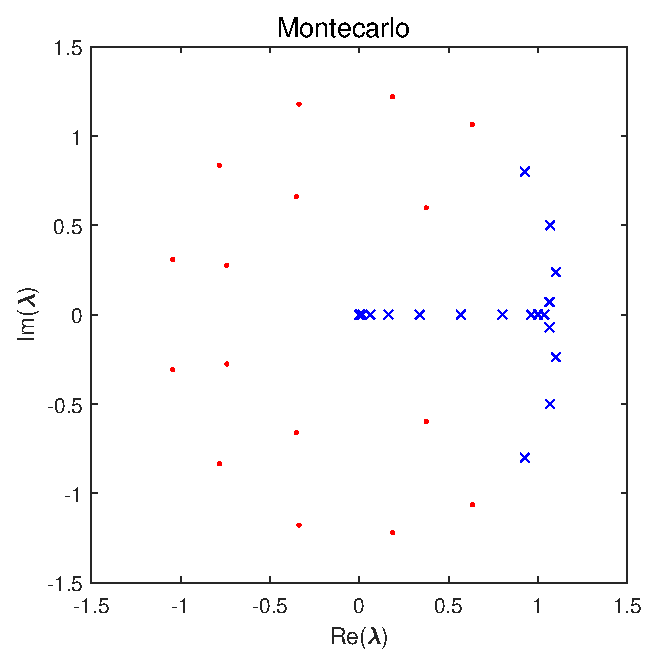
\includegraphics[width=0.25\linewidth]{../code/figures/gauss_map/ResDMD_Montecarlo.eps}
    \hspace*{\fill}
    \includegraphics[width=0.25\linewidth]{../code/figures/gauss_map/ResDMD_Riemann.eps}
    \hspace*{\fill}
    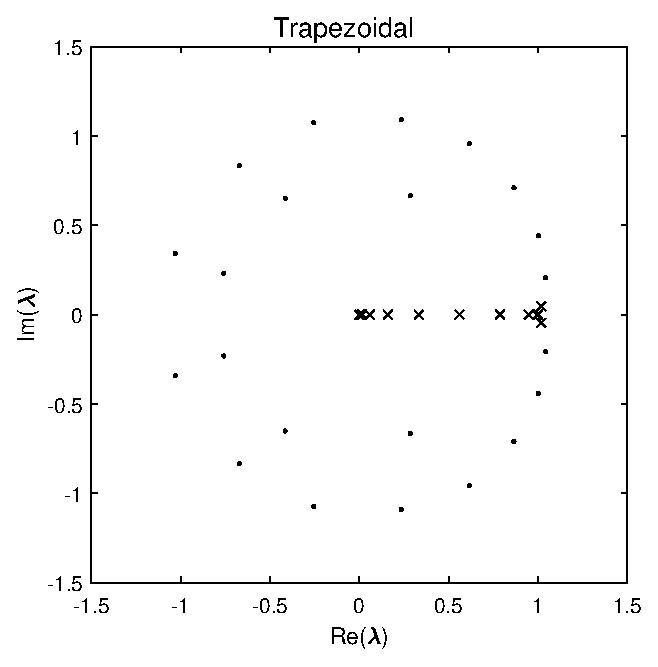
\includegraphics[width=0.25\linewidth]{../code/figures/gauss_map/ResDMD_Trapezoidal.eps}
    \hspace*{\fill}
    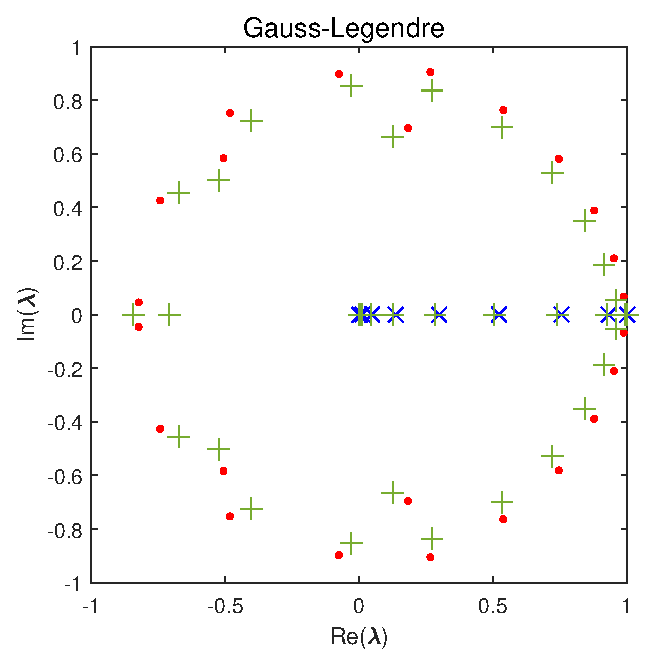
\includegraphics[width=0.25\linewidth]{../code/figures/gauss_map/ResDMD_Gauss-Legendre.eps}
    \hspace*{\fill}
}
\caption{Approximations of the eigenvalues of the Koopman Operator associated with the Gauss iterated map computed with the EDMD algorithm (magenta dots and blue crosses), using different quadrature rules. The approximated eigenvalues are computed using $K=40$ observables and the blue crosses indicate the eigenvalues retained by ResDMD, with tolerance $\varepsilon = 0.01$.}
\label{fig_resdmd_quadrature_comparison}
\end{figure}

\begin{figure}[h]
\makebox[\textwidth][c]{
    \begin{subfigure}{0.45\textwidth}
        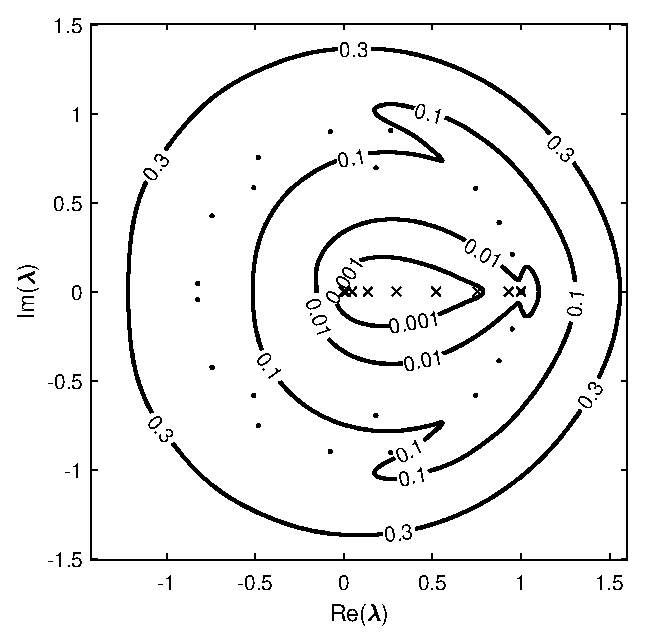
\includegraphics[width=\linewidth]{../code/figures/gauss_map/pseudospectra_contour.eps}
        \caption{Pseudospectral contours}
        \label{gauss_contours}
    \end{subfigure}\hspace*{\fill}
    \begin{subfigure}{0.45\textwidth}
        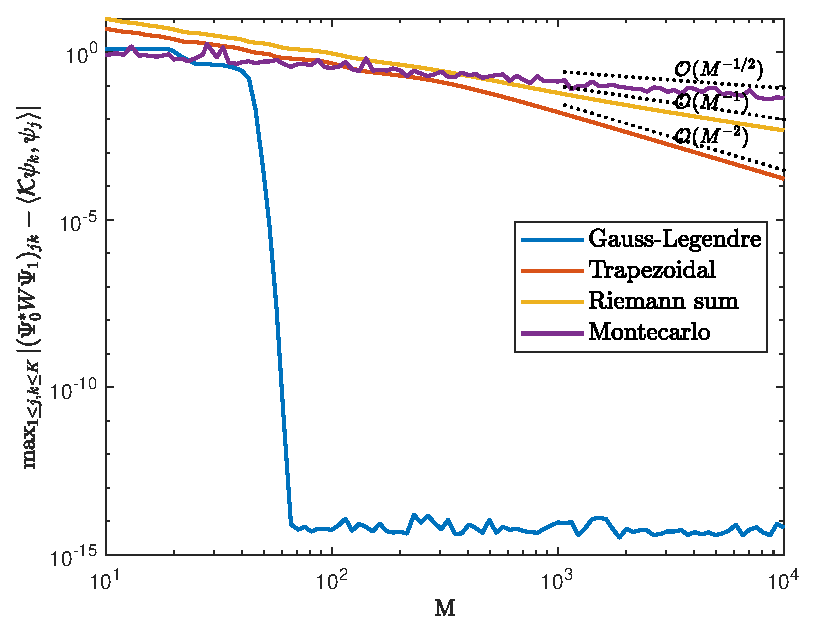
\includegraphics[width=\linewidth]{../code/figures/gauss_map/Galerkin_convergence.eps}
        \caption{Convergence of the quadrature rules}
        \label{gauss_convergence}
    \end{subfigure}\hspace*{\fill}
    }
    \caption{Contour lines of the $\varepsilon$-pseudospectrum for $\varepsilon = 0.3,\,0.1,\,0.01,\,0.001$ computed using \Cref{alg_pseudospectrum} with dictionary of $K=40$ observables (\Cref{gauss_contours}) and convergence of one of the approximated integrals for the different quadrature rulesm measured as $\max_{1\leq j,k \leq K} \abs{(\Psi_0^* W \Psi_1)_{jk} - \langle\mathcal{K}\psi_k, \psi_j\rangle}$ (\Cref{gauss_convergence}).}
    \label{gauss_pseudospectrum_convergence}
\end{figure}

\subsection{Nonlinear pendulum}
Let us consider the continous-time dynamical system of the nonlinear pendulum. The state variable is $\vb{x} = (x_1, x_2) = (\theta, \dot{\theta}) \in \Omega = [-\pi, \pi]_{\text{per}} \times \R$ and the differential equation governing the motion is
\begin{equation}
    \label{pendulum_equation}
    \dot{\vb{x}} = 
    \begin{bmatrix}
    \dot{x}_1 \\
    \dot{x}_2
    \end{bmatrix} = 
    \begin{bmatrix}
    x_2 \\
    -\sin(x_1)
    \end{bmatrix}.
\end{equation}
We consider the corresponding discrete-time dynamical system with time-step $\Delta_t = 0.5.$ and the associated Koopman Operator. The system is Hamiltonian and hence the Koopman Operator is unitary \cite{koopman_hamiltonian_1931}.

The choice of the dictionary of observables is now more complex, because the function governing the motion is vector-valued (with two components) and periodic in the first component. Since the motion is periodic in motion is periodic in $x_1\in[-\pi,\pi]_{\text{per}}$, it is natural to use the Fourier basis $\{e_n\}_{n\in\mathbb{Z}}$ in $x_1$ to describe the motion in this direction. Similarly, to approximate the motion in the direction of $x_2$ one might decide to use the Hermite functions $\{h_n\}_{n\in\mathbb{N}}$, which form a basis of the Hilbert space $L^2(\R)$. Therefore, we would ideally consider observables of the form $\phi(x_1, x_2) = \sum_{n\in\mathbb{Z},\,m\in\mathbb{N}} \alpha_{n,m} e_n(x_1)\cdot h_m(x_2)$ for some coefficients $\{\alpha_{n,m}\}\in\C$. However, our dictionary of observables must be finite and we need to decide a criterion to truncate the sum. Observe that there isn't a natural ordering as if the indices were in $\mathbb{N}$ or $\mathbb{Z}$. Since we want to be able to approximate the (components of the) full state observable, it is important to have the indices $\{(n,0)\}_{n=0}^{n_{\max}}$ and $\{(0,m)\}_{m=-m_{\max}}^{m_{\max}}$ with $n_{\max},\,m_{\max}$ as high as possible. Selecting the indices in the rectangle $\{(n,m)\,:\,-n_{\max}\leq n\leq n_{\max},\,\, 0\leq m\leq m_{\max}\}$ would make the size of the dictionary grow too fast in $n_{\max}$ and $m_{\max}$, thus we use an hyperbolic cross approximation \cite{dung_hyperbolic_2017}, i.e. we select the indices in the hyperbolic cross $\{(n,m)\,:\, \max(n,1)\cdot \max(m,1)\leq N \}$, where $N$ is called the order of the hyperbolic cross approximation.

Using \Cref{alg_pseudospectrum} we compute an approximation of the $\varepsilon$-pseudospectrum for $\varepsilon = 0.25$, first using $K=193$ observables and $M = 10^4$ data points, then employing $K=1265$ and $M = 9 \times 10^4$. As the size $K$ of the dictionary increases, the approximation of the $\varepsilon$-pseudospectrum approaches the annulus with internal radius 0.75 and external radius 1.25(see \Cref{pendulum_pseudospectrum}). We also compute approximation of the eigenfunctions associated with the eigenvalues $\lambda = \exp(0.4932 i), \,\lambda = \exp(0.9765 i), \,\lambda = \exp(1.4452 i), \,\lambda = \exp(1.8951 i), \,$ (see \Cref{pendulum_phase_portraits}).

\textcolor{red}{COMMENT MORE ON THE RESULTS(?)}

\begin{figure}[h]
\makebox[\textwidth][c]{
    \begin{subfigure}{0.45\textwidth}
        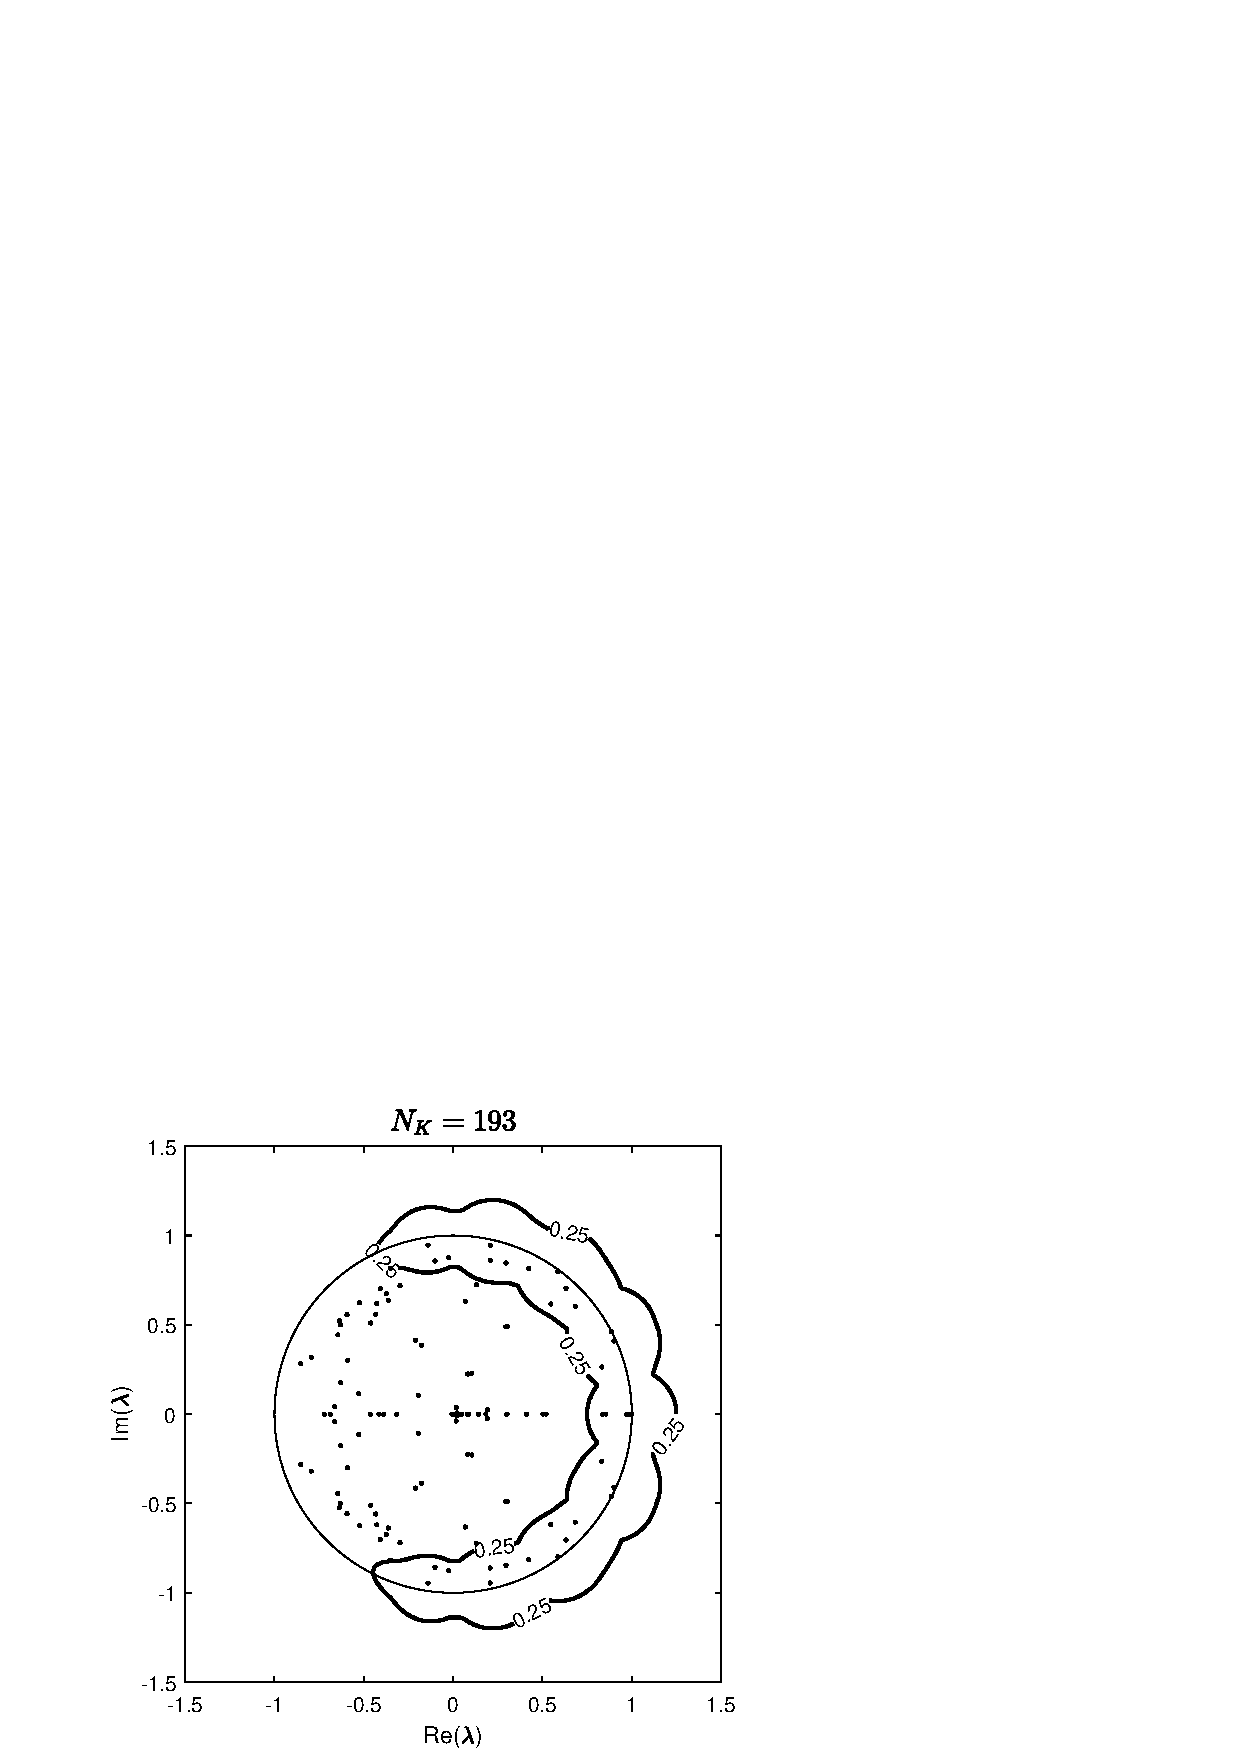
\includegraphics[width=\linewidth]{../code/figures/pendulum/pendulum_N193.png}
    \end{subfigure}\hspace*{\fill}
    \begin{subfigure}{0.45\textwidth}
        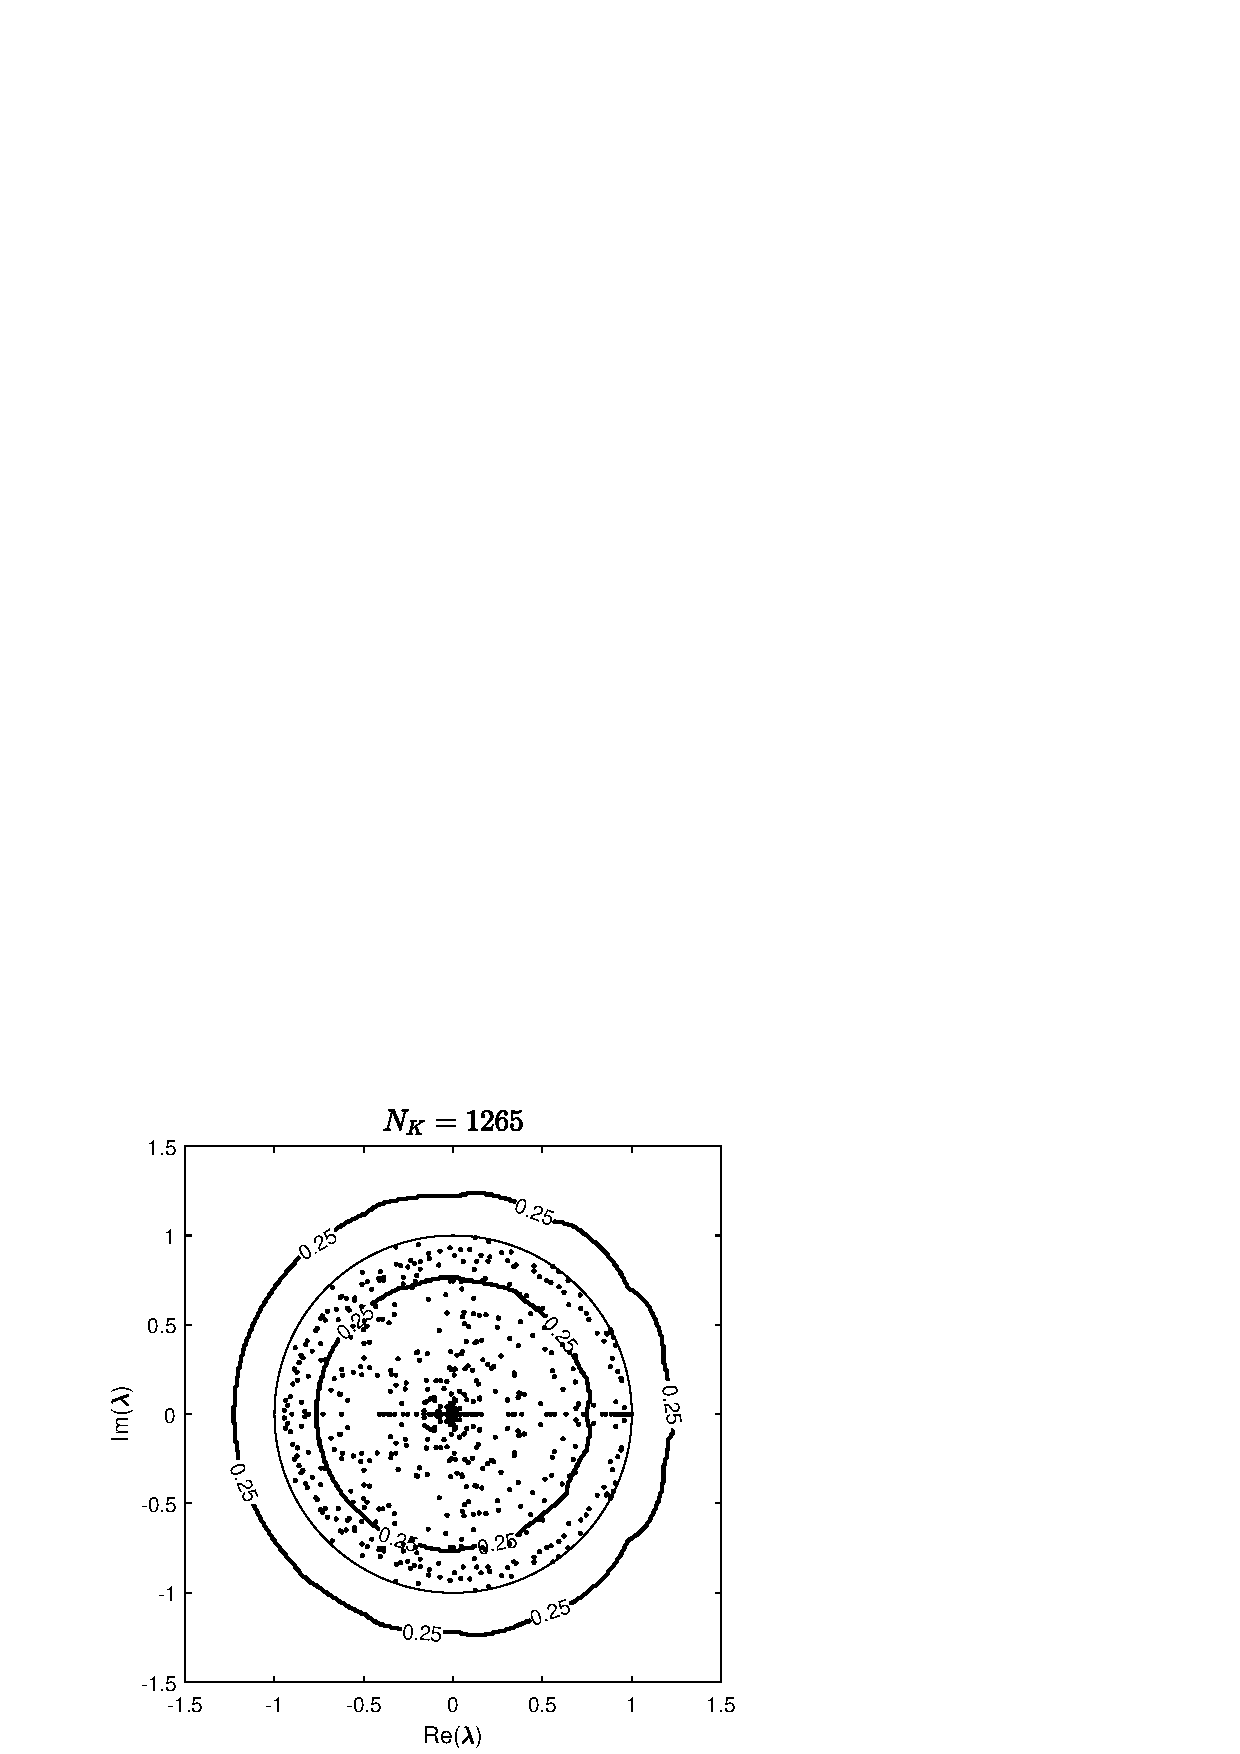
\includegraphics[width=\linewidth]{../code/figures/pendulum/pendulum_N1265.png}
    \end{subfigure}\hspace*{\fill}
        }
    \caption{Contour lines of the $\varepsilon$-pseudospectrum for $\varepsilon = 0.25$ computed using \Cref{alg_pseudospectrum} with hyperbolic cross approximation. On the left the approximation obtained using a dictionary of $K=193$ observables and $M = 10^4$ data points, on the right the one obtained with $K=1265$ and $M = 9 \times 10^4$.}
    \label{pendulum_pseudospectrum}
\end{figure}

\begin{figure}[h]
\centering
\makebox[\textwidth][c]{
        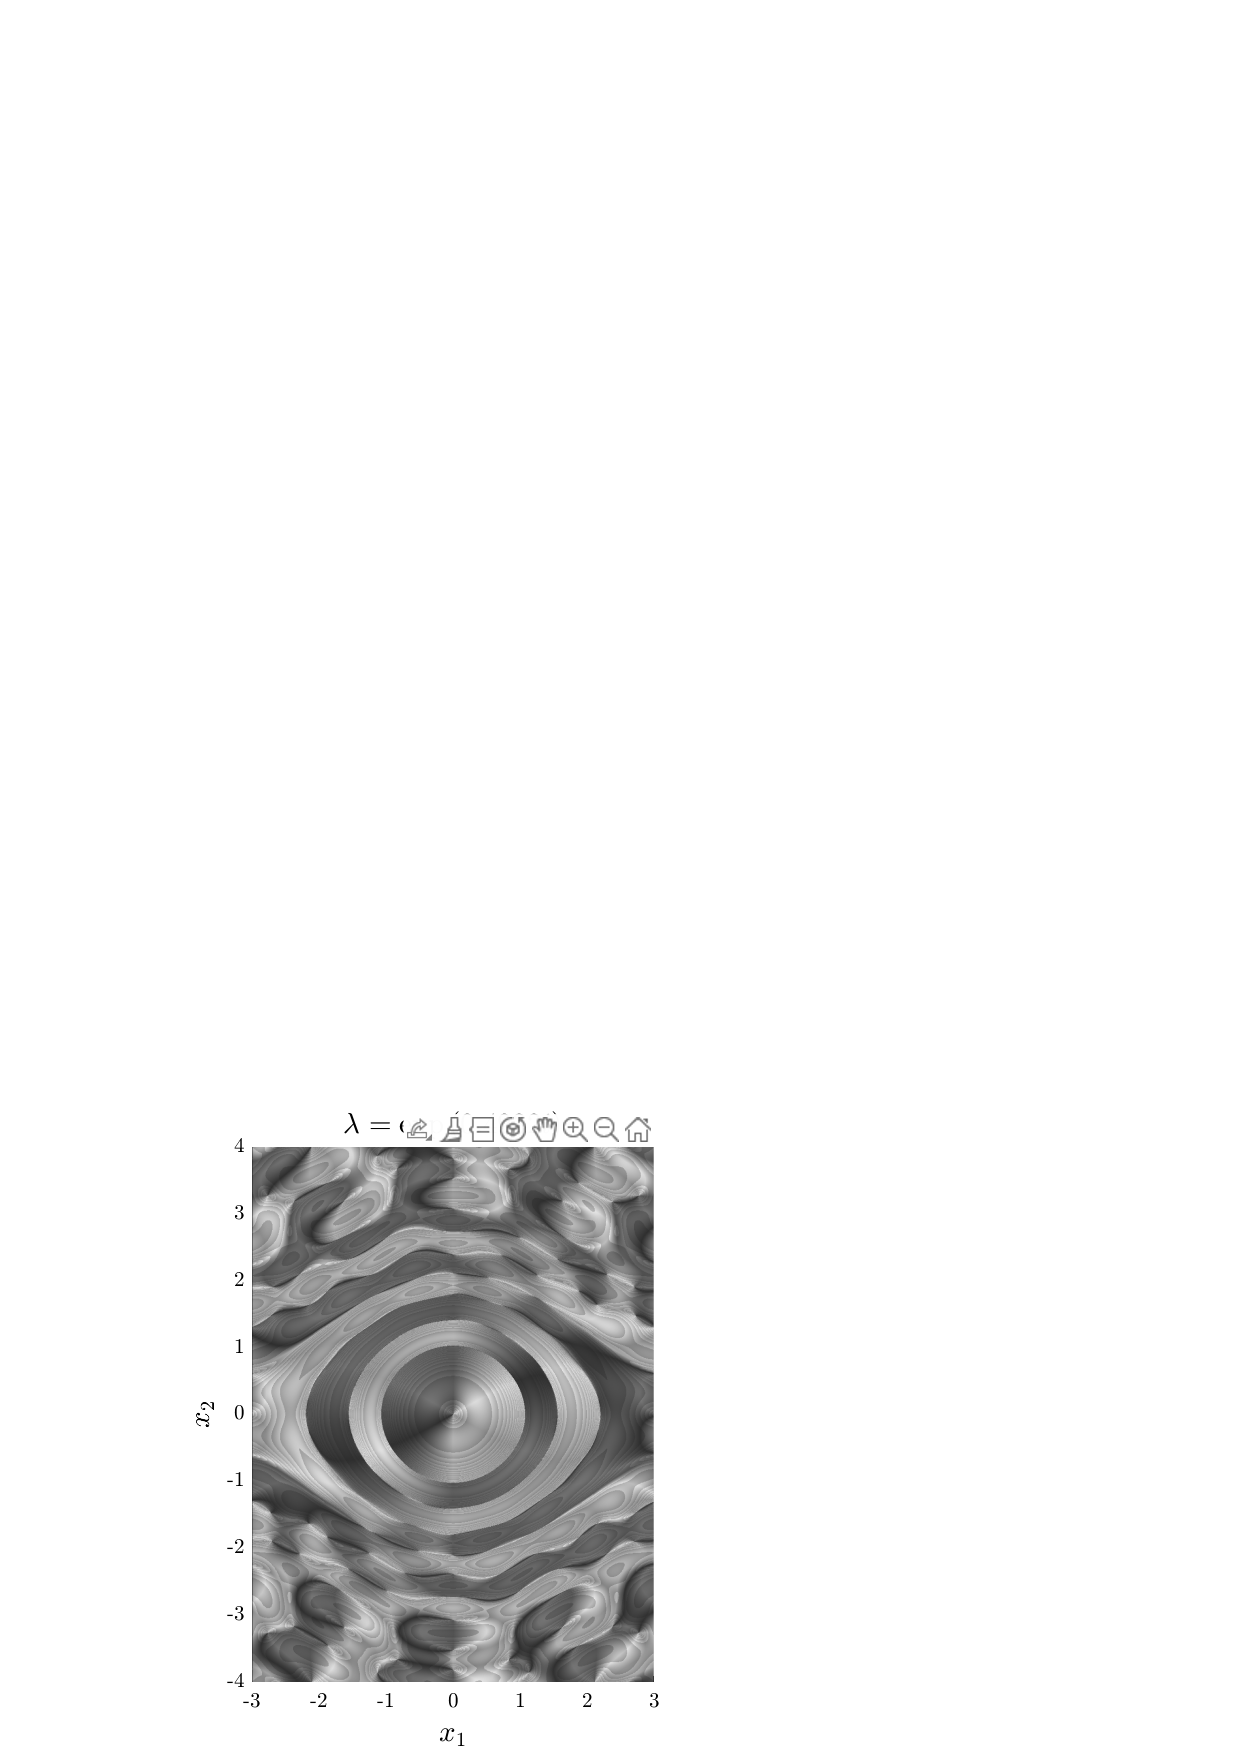
\includegraphics[width=0.25\linewidth]{../code/figures/pendulum/phase_portrait_4932.png}
        \hspace*{\fill}
        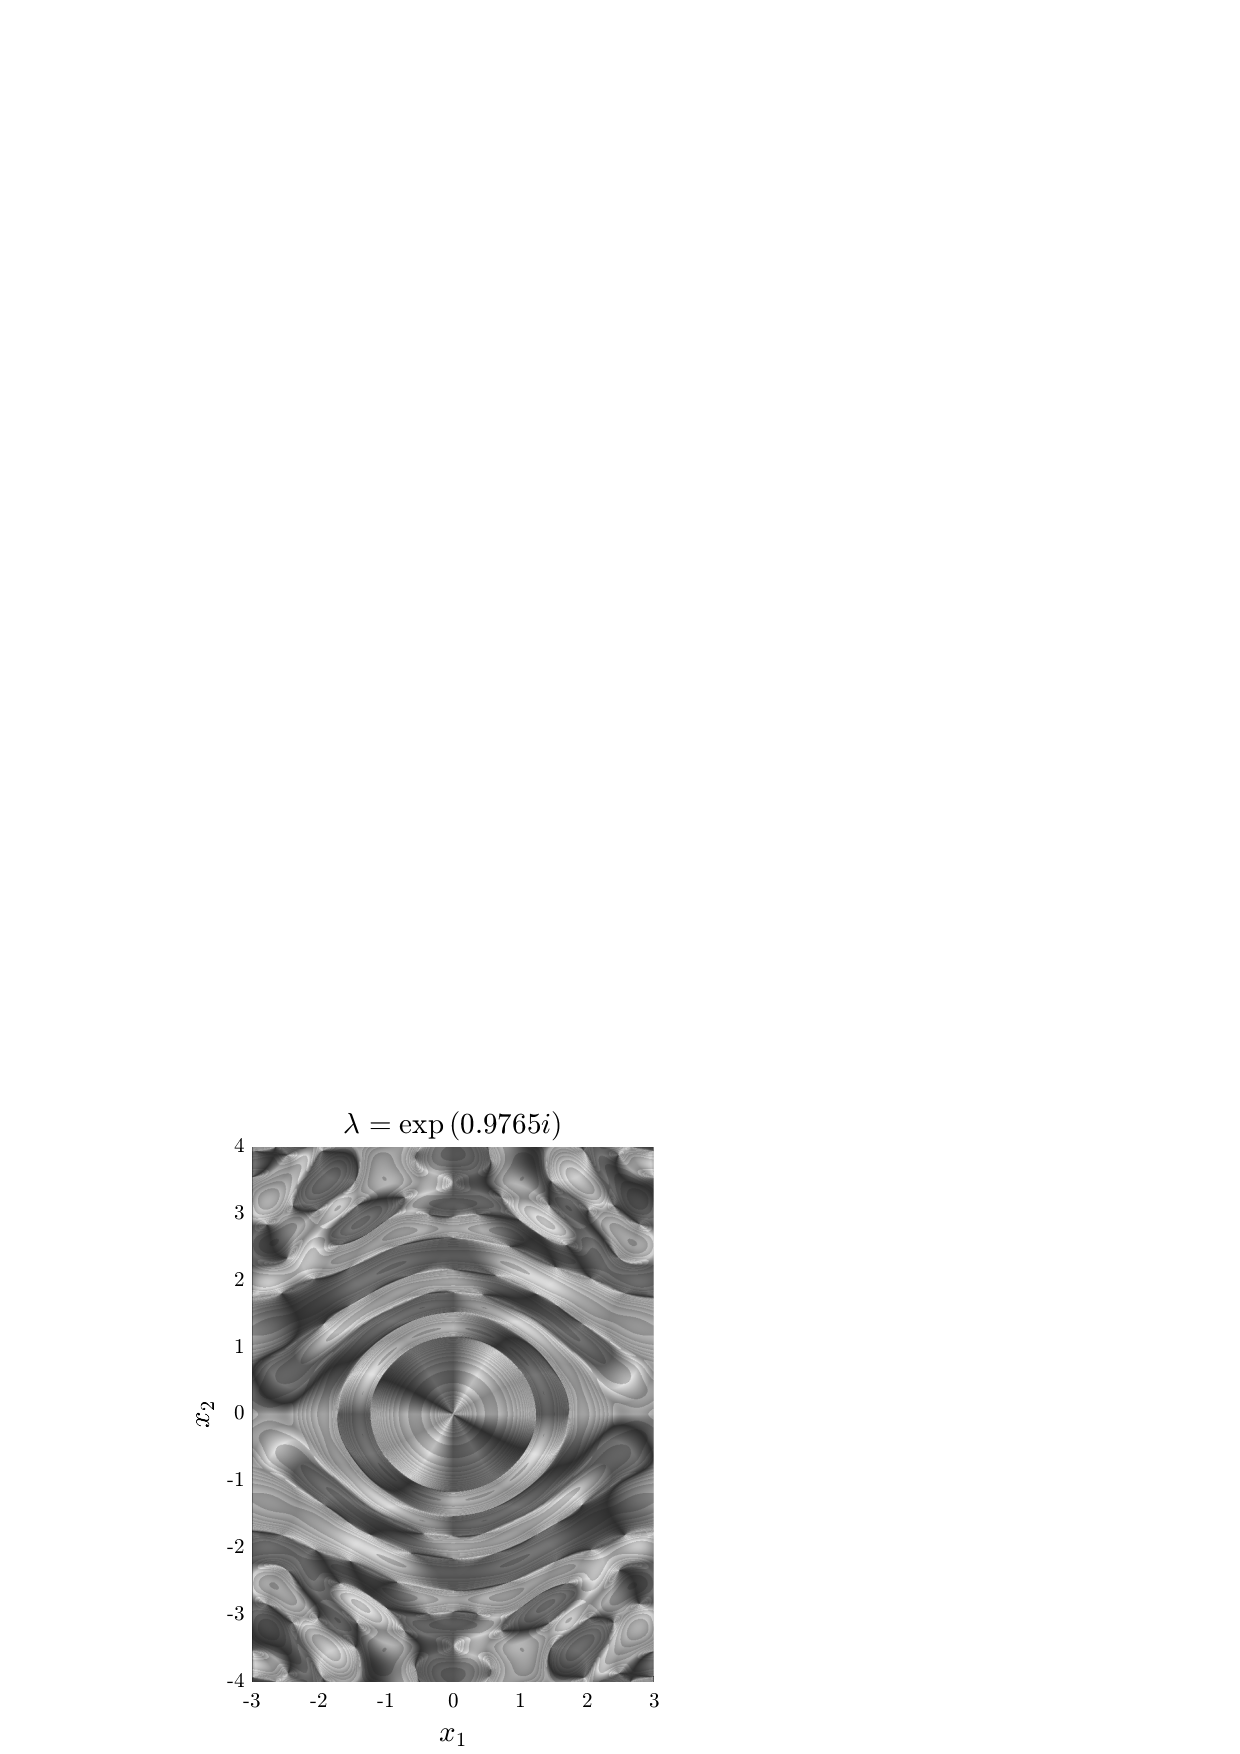
\includegraphics[width=0.25\linewidth]{../code/figures/pendulum/phase_portrait_9765.png}
        \hspace*{\fill}
        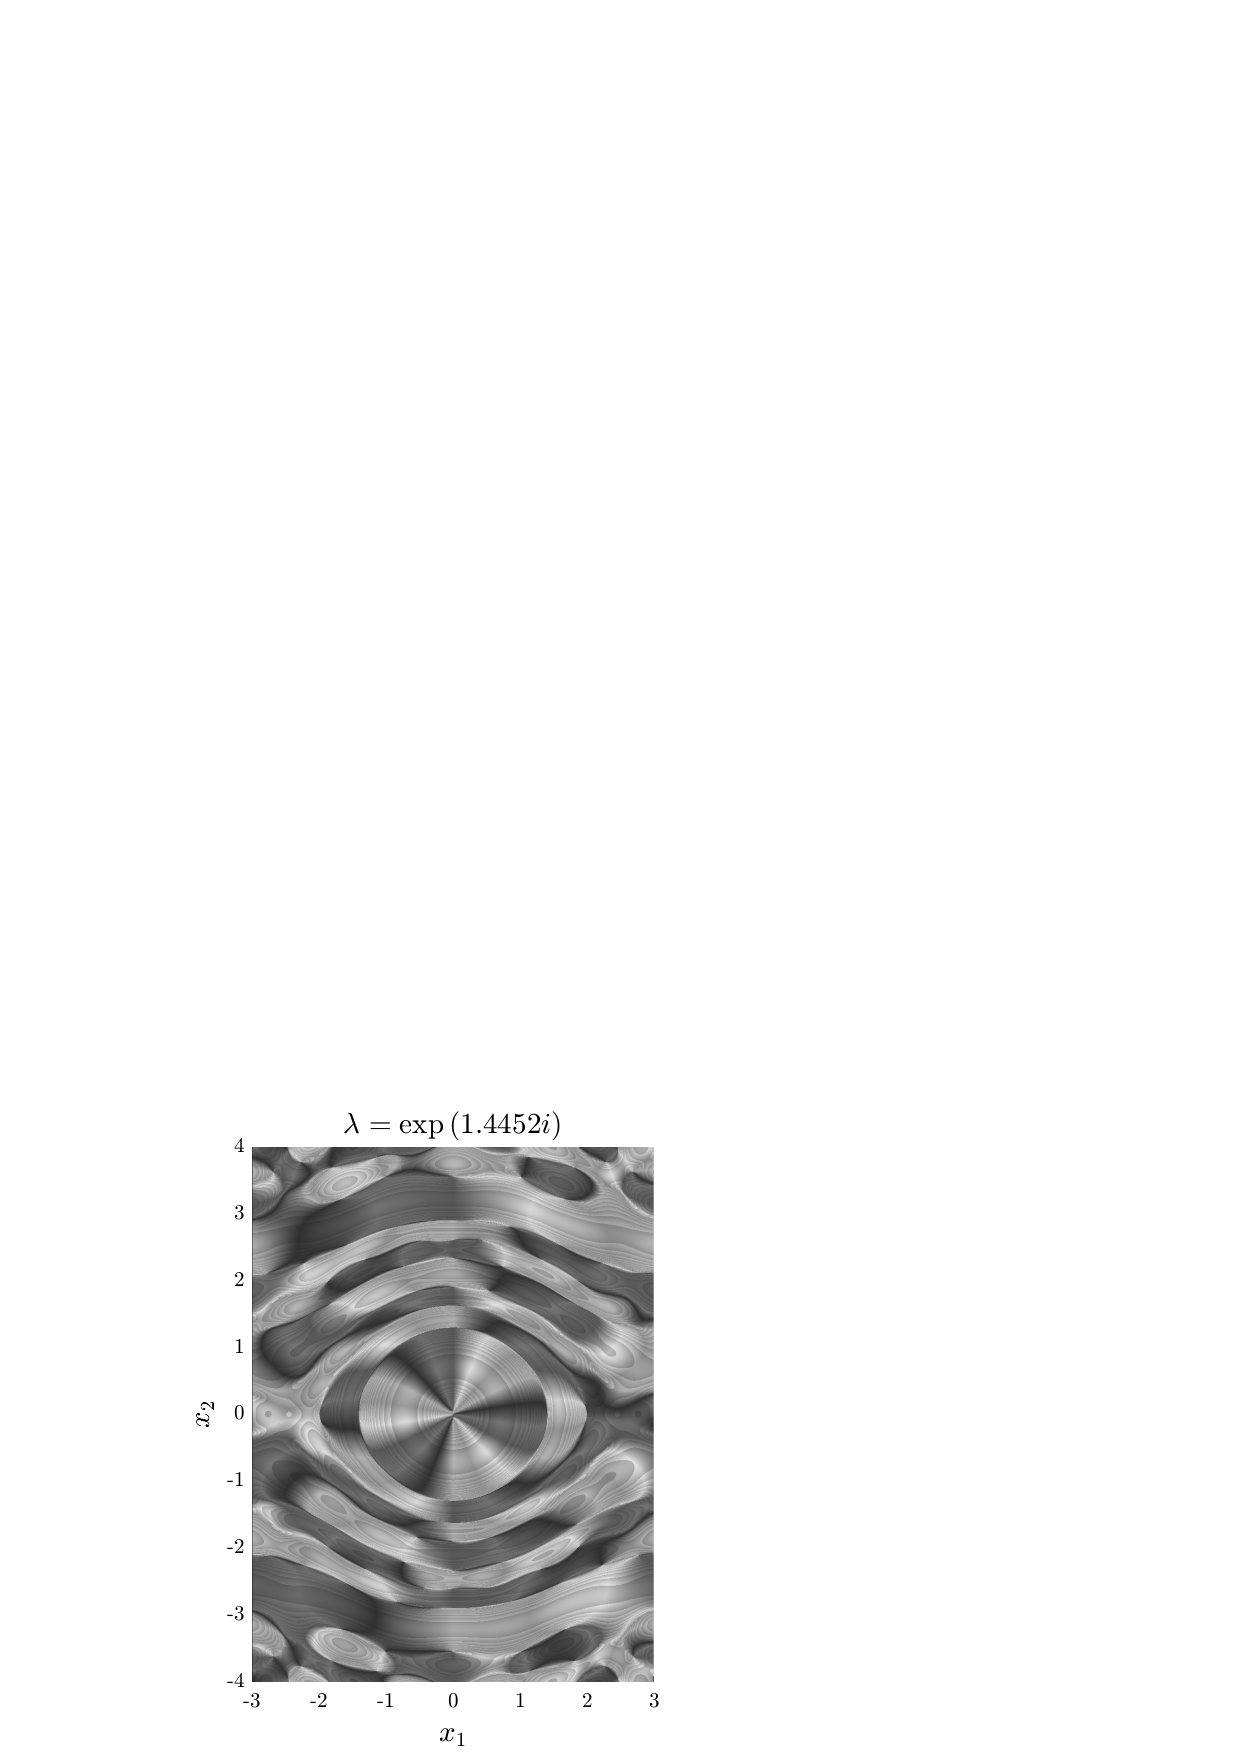
\includegraphics[width=0.25\linewidth]{../code/figures/pendulum/phase_portrait_14452.png}
        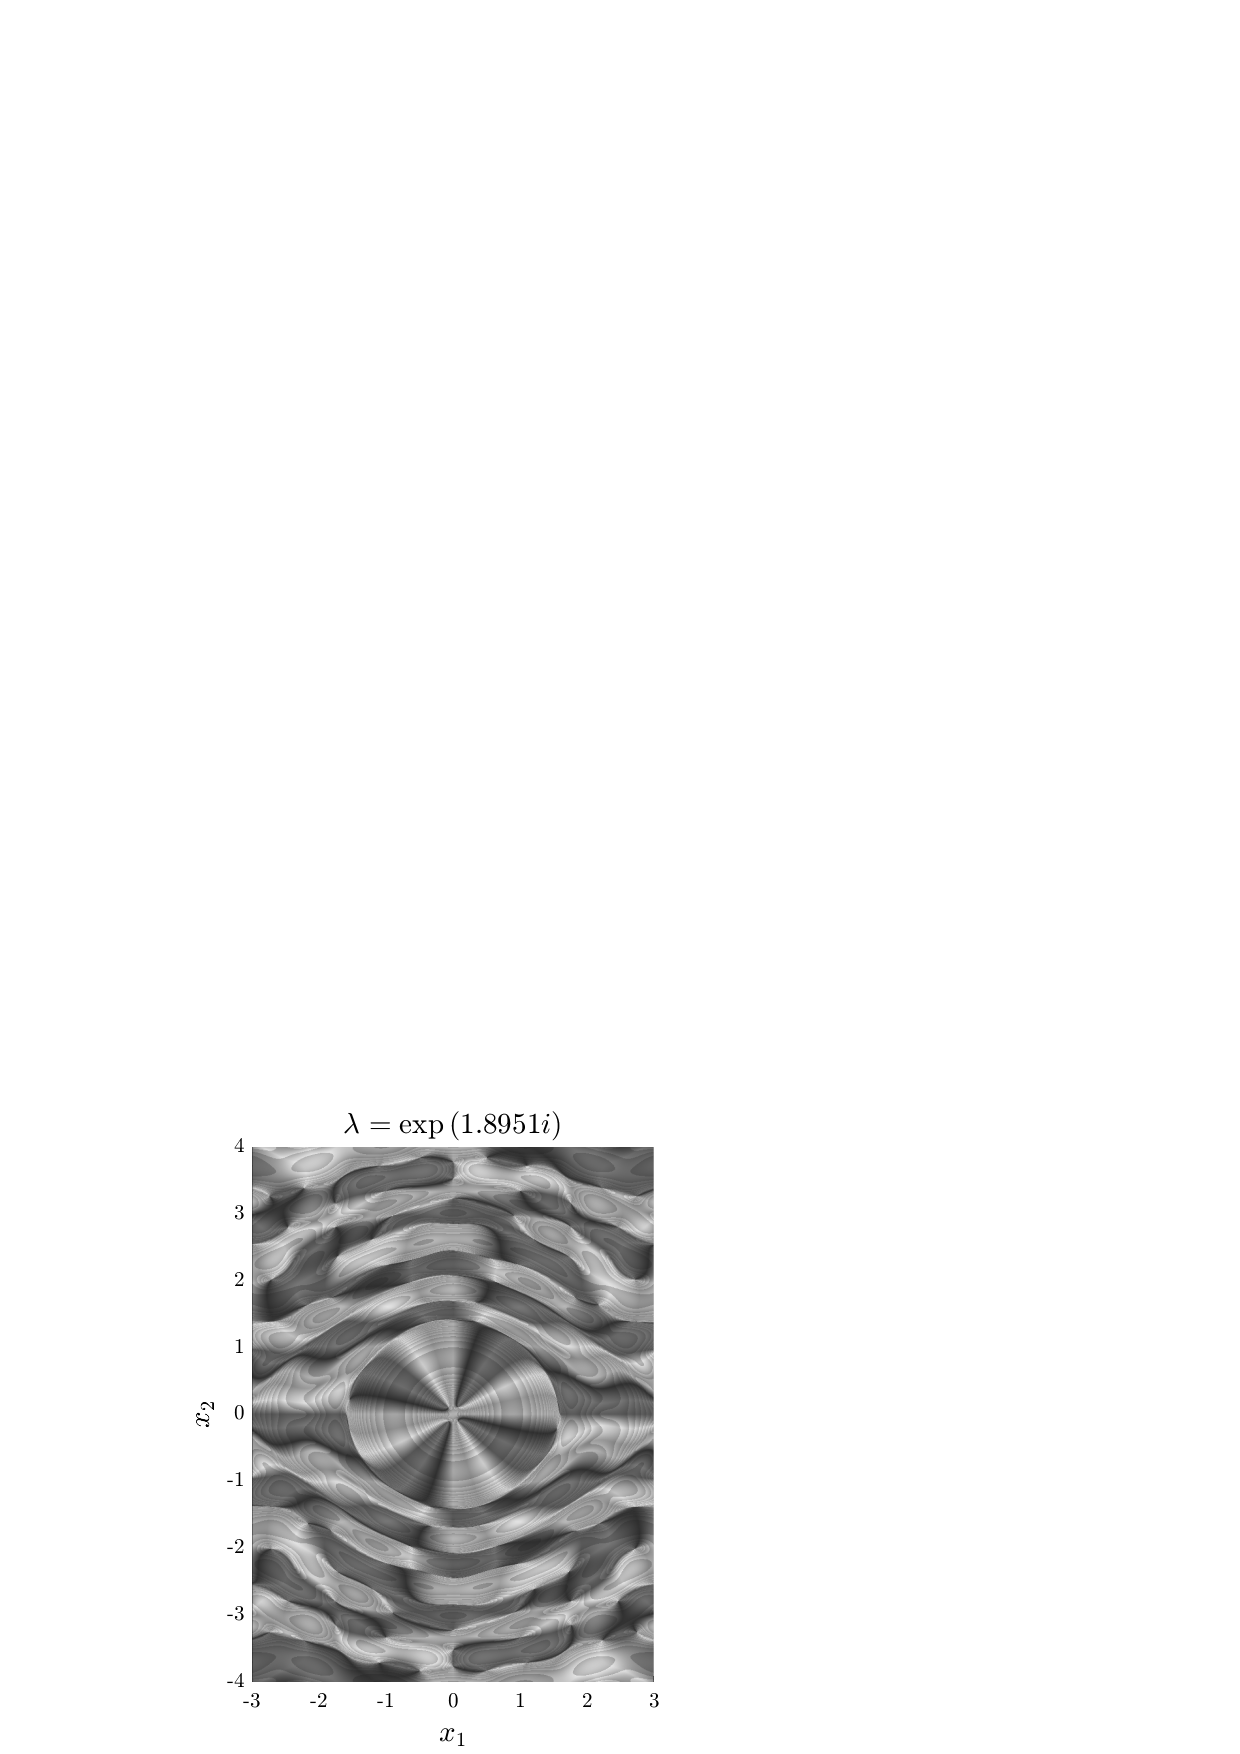
\includegraphics[width=0.25\linewidth]{../code/figures/pendulum/phase_portrait_18951.png}
        \hspace*{\fill}}
        \caption{Phase portraits of the approximate eigenfunctions of the nonlinear pendulum, where the color illustrates the complex argument of the eigenfunction. Lines of constant modulus are plotted as shadowed steps.}
        \label{pendulum_phase_portraits}
\end{figure}